\documentclass[letterpaper,10pt]{article}
\usepackage{graphicx}
\usepackage{osameet2}
\usepackage{amsmath,amssymb}


\begin{document}
\title{Objective-First Design of Nanophotonic Waveguide Couplers}
\author{Jesse Lu and Jelena Vu\v{c}kovi\'{c}}
\address{Stanford University, Stanford, California, USA.}
\email{jesselu@stanford.edu}

\maketitle
\begin{abstract}
We introduce an ``objective-first'' approach to the design of
    nanophotonic waveguide couplers.
Our method is
    computationally fast (20 minutes on a single-core personal computer), 
    requires no trial-and-error,
    does not require guessing a good starting design,
    can be applied to arbitrary waveguide modes,
    and generates devices with high coupling efficiencies (typically 95\%)
    and small footprints (1-4 square vacuum wavelengths).
\end{abstract}
\ocis{230.7370, 130.3990.}

\begin{thebibliography}{99}
\bibitem{fibergrating} Y. Tang, Z. Wang, L. Wosinski, U. Westergren, and S. He,
    ``Highly efficient nonuniform grating coupler for silicon-on-insulator 
    nanophotonic circuits,''
    Opt. Lett. \textbf{35}, 1290-1292 (2010)
\bibitem{ridge}  K. K. Lee, D. R. Lim, L.C. Kimerling, J. Shin, and F. Cerrina, 
    ``Fabrication of ultralow-loss Si/SiO2 waveguides by roughness reduction,''
    Opt. Lett. \textbf{26}, 1888-1890 (2001)
\bibitem{pcslow} Y. A. Vlasov, M. O'Boyle, H. F. Hamann, and S. J. McNab,
    ``Active control of slow light on a chip with photonic crystal waveguides,''
    Nature \textbf{438}, 65-69 (2005)
\bibitem{slotfocus} M. Lipson, 
    ``Guiding, Modulating, and Emitting Light on 
    Silicon-Challenges and Opportunities,'' 
    J. Lightwave Technol. \textbf{23}, 4222-4238 (2005) 
\bibitem{active} J. Van Campenhout, P. Rojo Romeo, P. Regreny, C. Seassal, 
    D. Van Thourhout, S. Verstuyft, L. Di Cioccio, J.-M. Fedeli, 
    C. Lagahe, and R. Baets, 
    ``Electrically pumped InP-based microdisk lasers integrated with a 
    nanophotonic silicon-on-insulator waveguide circuit,'' 
    Opt. Express \textbf{15}, 6744-6749 (2007) 
\bibitem{metallic} L. Tang, S. E. Kocabas, S. Latif, A. K. Okyay, 
    D. S. Ly-Gagnon, K. C. Saraswat and D. A. B. Miller, 
    ``Nanometre-Scale Germanium Photodetector Enhanced by a 
    Near-Infrared Dipole Antenna,'' 
    Nature Photonics \textbf{2}, 226 – 229 (2008) 
\bibitem{fwadia} V. R. Almeida, R. R. Panepucci, and M. Lipson, 
    ``Nanotaper for compact mode conversion,'' 
    Opt. Lett. \textbf{28}, 1302-1304 (2003) 
\bibitem{wwadia} S. G. Johnson, P. Bienstman,  M. A. Skorobogatiy, 
    M. Ibanescu1, E. Lidorikis, and J. D. Joannopoulos,
    ``Adiabatic theorem and continuous coupled-mode theory for 
    efficient taper transitions in photonic crystals,''
    Phys. Rev. E \textbf{66}, 066608 (2002)
\bibitem{deriv} F. Wang, J. S. Jensen, O. Sigmund, 
    ``Robust topology optimization of photonic crystal waveguides with 
    tailored dispersion properties.'' 
    J. Opt. Soc. Am. B \textbf{28}, 387-397 (2011)
\bibitem{boydbook} S. Boyd, and L. Vandenberghe, 
    \emph{Convex Optimization} 
    (Cambridge University Press, 2004)
\bibitem{prevwork} J. Lu, S. Boyd, and J. Vuckovic, 
    ``Inverse design of a three-dimensional nanophotonic resonator,''
    Opt. Express \textbf{19}, 10563-10570 (2011) 
\bibitem{code} \url{www.github.com/JesseLu/objective-first}
\end{thebibliography}

\section{Motivation}

% Why is waveguide mode conversion important?
\subsection{The importance of waveguide mode conversion}
Optical mode conversion, 
    the efficient transfer of photons from one guided mode to another,
    is a fundamental requirement in nanophotonics.
Efficient conversion between waveguides modes
    is critical in the many cases, including:
    \begin{enumerate}
        \item Coupling to and from optical fiber\cite{fibergrating}, 
        to communicate with the outside world.
    \item Coupling between various nanophotonic waveguides, 
        since different waveguides are best suited for different applications.
        For example, ridge waveguides seem ideal for 
            low-loss transport\cite{ridge},
            but other waveguides, 
            such as photonic crystal waveguides or slot waveguides,
            may be better suited for slow-light\cite{pcslow} 
            or nonlinear optical devices based on 
            localized field intensities\cite{slotfocus}.
    \item Coupling between different materials systems such as
       passive, active\cite{active}, and metallic\cite{metallic} devices. 
    \end{enumerate}
Although efficient waveguide coupling is essential in any nanophotonic system,
    practical methods to design couplers have not yet been developed.

% Why are current solutions insufficient?
\subsection{Approaches to designing waveguide couplers}
% Brute force
Of the design strategies currently available,
    brute-force parameter search is the most often employed 
    because of its sheer simplicity.
Although it may be suitable for tuning existing designs,
    the parameter space for most practical devices is simply too large
    for such a strategy to be tractable.

% Adiabatic mode conversion (large devices, symmetry breaking)
Adiabatic mode conversion strategies have been succesful
    for certain fiber-waveguide\cite{fwadia} and 
    waveguide-waveguide\cite{wwadia} couplers,
    even if the resulting devices often require large footprints.
However, adiabatic approaches cannot be used in many important cases 
    such as coupling in the out-of-plane direction, or
    coupling between modes of opposite symmetry.

% Local optimization
On the other hand, optimization methods based on local topological derivatives 
    seem very promising\cite{deriv}
    in that they are both much faster than brute-force methods and
    more adaptable than adiabatic strategies.
However, these methods still carry a significant computational burden 
    in that every updated design must be simulated at least once.
Also, there is a significant burden for the user from whom
    a good initial design is usually required.


% How does your algorithm solve this problem?
% \subsection{Advantages of objective-first design}
In contrast, our method
\begin{itemize}
    \item does not employ brute-force parameter searches,
    \item does not require a good initial design,
    \item is computationally fast (no simulations required),
    \item generates couplers between seemingly arbitrary waveguide modes, and
    \item can generate these couplers within a very small footprint. 
\end{itemize}
We outline the general design strategy,
    as well as how it is applied to coupler design, in the section below.

\section{Methods}
% What is objective-first optimization?
\subsection{Objective-first optimization}
The typical approach to designing physical structures can be formulated 
    in the following way, 
    where $x$ is the field variable and $p$ is the structure variable,
    \begin{subequations}\label{eq:adj}
    \begin{align} 
    \text{decrease} & \quad f(x) \label{eq:adj:obj} \\ 
    \text{subject to} & \quad g(x,p) = 0. \label{eq:adj:con}
    \end{align}
    \end{subequations}
Here, $f(x)$, the \emph{design objective}, 
    calculates the performance of the device 
    (e.g. amount of power not coupled to output mode); 
    while $g(x,p)$ is the underlying physical equation for the system
    (e.g. the electromagnetic wave equation).

In contrast, the objective-first formulation is
    \begin{subequations}\label{eq:ob1}
    \begin{align} 
    \text{decrease} & \quad \|g(x,p)\|^2 \label{eq:ob1:obj} \\ 
    \text{subject to} & \quad f(x) = 0, \label{eq:ob1:con}
    \end{align}
    \end{subequations}
    where $\|g(x,p)\|^2$ is the \emph{physics residual}.
We term this formulation ``objective-first''
    because the design objective is prioritized even above satisfying physics;
    specifically, we force our design to always exhibit the desired performance
    ($f(x) = 0$).

The differences between Eqs.~\ref{eq:adj} and \ref{eq:ob1} are:
\begin{enumerate}
    \item in Eq.~\ref{eq:adj:obj}, we attempt to decrease the design objective,
        while in Eq.~\ref{eq:ob1:con}, the design objective is kept at zero
        (i.e. we force the optimization to satisfy the design objective);
    \item in Eq.~\ref{eq:adj:con}, we always satisfy the underlying physics,
        while in Eq.~\ref{eq:ob1:obj}, physics is not necessarily satisfied,
            since the physics residual is generally non-zero
            (although the optimization is directed at minimizing this residual).
\end{enumerate}

Thus, the fundamental innovation in the objective-first approach
    is simply this:
    we forcibly impose the desired performance on the device at the expense of
    not perfectly satisfying the physical equation which governs its operation.

% What are the implications of the objective-first approach?
\subsection{Numerical implications of the objective-first approach}

While the differences between the design strategies presented in 
    Eqs.~\ref{eq:adj} and \ref{eq:ob1} are straightforward,
    the numerical implications are more subtle.

The first practical implication of the objective-first approach 
    is that the number of independent variables is increased to include
    both $x$ and $p$.
This occurs because in Eq.~\ref{eq:adj}, 
    the constraint that physics must be satisfied, $g(x,p)=0$, 
    essentially forces $x$ to be a dependent variable,
    since the choice of $p$ implicitly determines the value of $x$
    (there is generally a one-to-one mapping from $p$ to $x$).
In contrast, Eq.~\ref{eq:ob1} allows both $x$ and $p$ to vary independently,
    because the constraint, $f(x)=0$, is only a function of $x$.

Secondly, the amount of computation needed to enforce the constraint is
    drastically reduced in our objective-first approach.
This is because Eq.~\ref{eq:adj} requires a full solution of $g(x,p)=0$
    (i.e. a full simulation of the structure, $p$) to compute $x$.
In contrast, the constraint $f(x)=0$ in Eq.~\ref{eq:ob1} 
    can often be enforced with a trivial amount of computation (as shown below).

Lastly, the objective-first approach eliminates the need for even a reasonable
    initial design.
Generally, methods based on Eq.~\ref{eq:adj} require an initial design which
    already provides some limited functionality
    (e.g. a coupler which already transfers 
    a non-zero amount of power to the desired output mode).
In constrast, out method, based on Eq.~\ref{eq:ob1}, performs just as well
    when started from a completely non-functional design 
    (e.g. a coupler which transfers no power into the desired output mode).

% How is it applied to waveguide coupler design?
\subsection{Objective-first approach to waveguide coupler design}
We now apply the objective-first approach to the problem of designing 
    two-dimensional nanophotonic waveguide couplers.

We choose to work in the two-dimensional transverse electric mode,
    which only couples $E_x$, $E_y$, and $H_z$ ($E_z, H_x, H_y = 0$),
    since it is most relevant for on-chip devices.
We choose to use $H_z$ as the field variable ($x$ in Eq.~\ref{eq:ob1}), 
    and $\epsilon^{-1}$ (inverse of the permittivity) 
    as the structure variable $p$.
This results in the following representation of the physics residual, 
    based on the time-harmonic electromagnetic wave equation without sources;
    \begin{equation}
    \|g(H_z, \epsilon^{-1})\|^2 = 
    \| \nabla \times \epsilon^{-1} \nabla \times H_z - \mu_0 \omega^2 H_z \|^2,
    \end{equation}
    where $\omega$ is the angular frequency,
    and $\mu_0$ is the permeability of free-space.

For the design objective, we choose a boundary-value formulation
    based on $H_z^\text{perfect}$,
    where $H_z^\text{perfect}$ is constructed 
    of the exact input and output waveguide modes at the input and output ports
    of the optimization region (where the coupler will be placed),
    repectively, and of zero-amplitude fields at the unused ports.

% \begin{figure}[htbp]
%     \centering
%     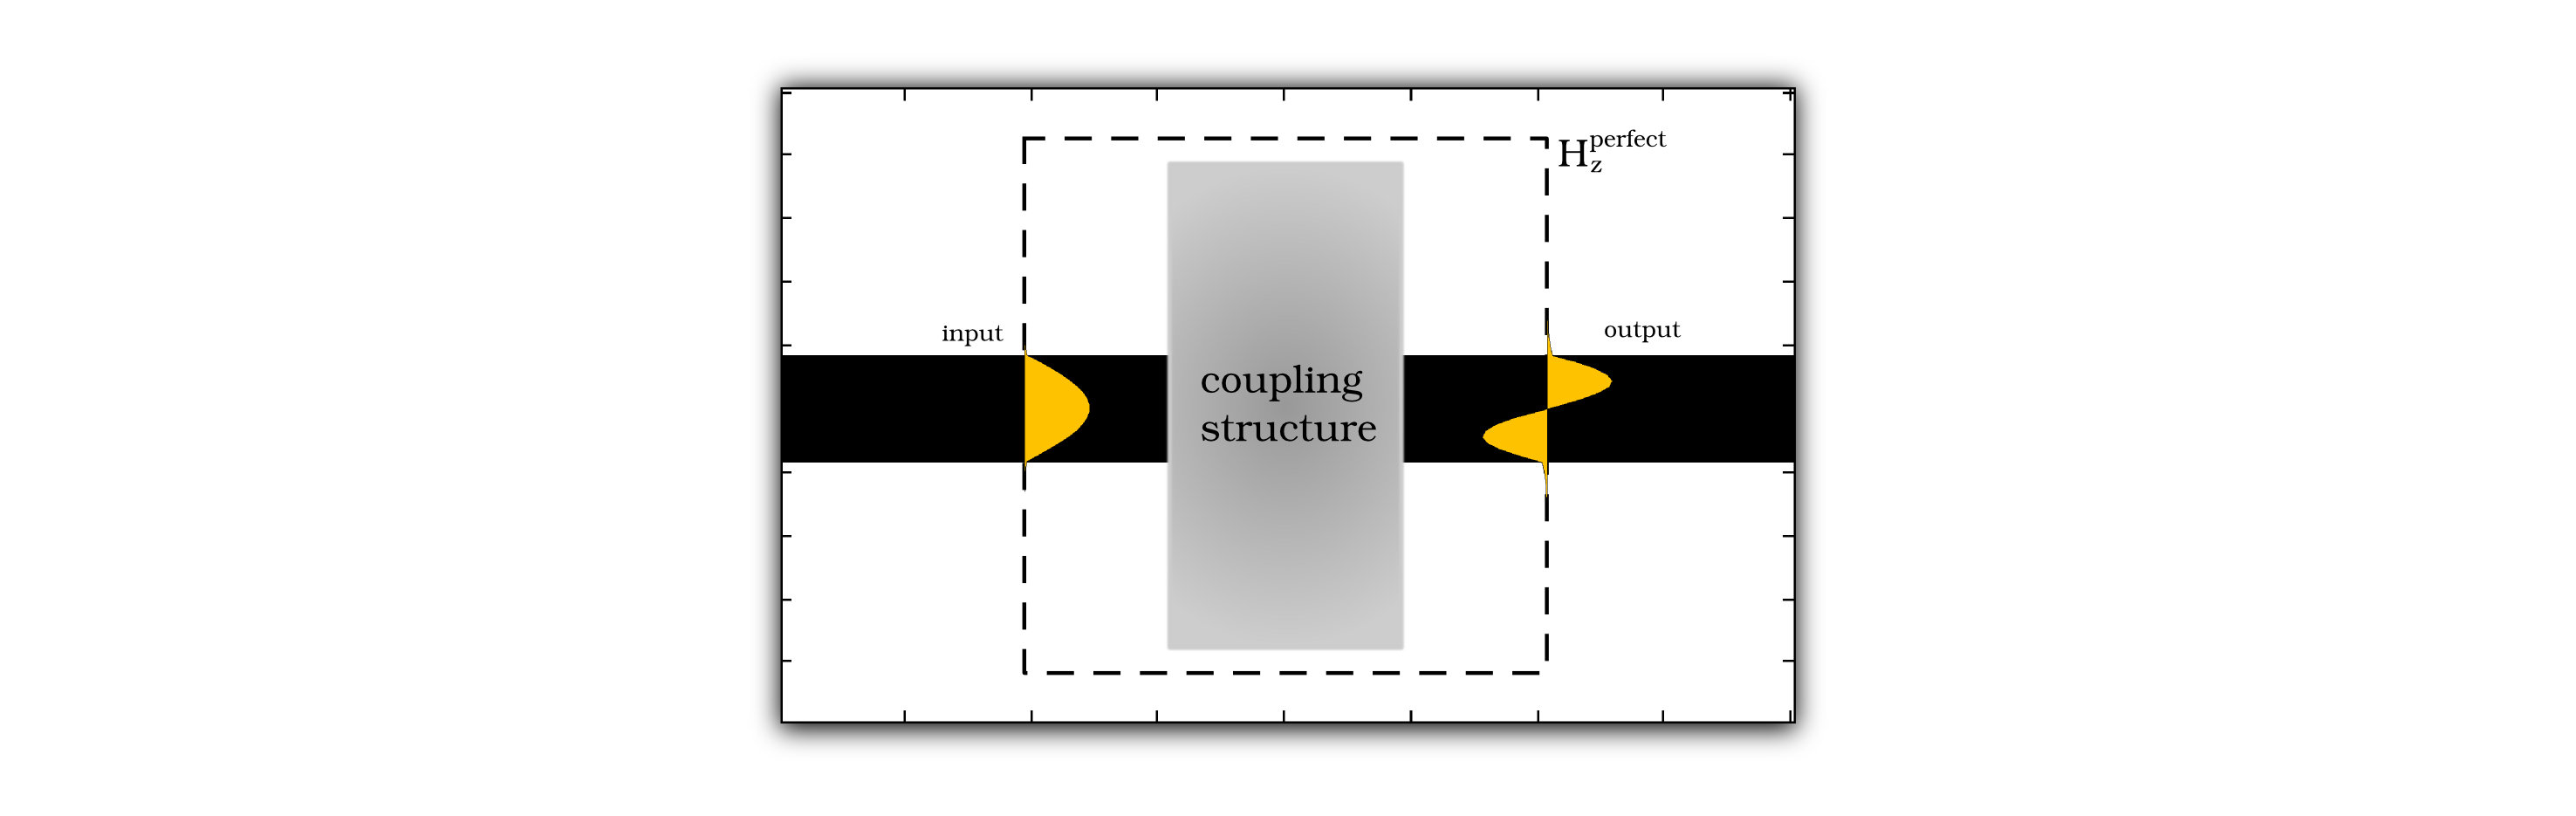
\includegraphics[width=\textwidth]{intro} 
%     \caption{Boundary-value formulation of the design objective.
%         The values of $H_z^\text{perfect}$, 
%             defined along the dashed box surrounding the design area
%             (coupling structure), 
%             are shown in orange (color online).
%         The values of $H_z^\text{perfect}$ along the top and bottom edges
%             of the dashed box are set to zero.
%         In this schematic, the fundamental and second-order waveguide modes
%             have been chosen as the input and output modes respectively.}
%     \label{fig:intro}
% \end{figure}

The mathematical form of the design objective is simply, 
    \begin{equation}
    f(H_z) = \begin{bmatrix}
        H_z - H_z^\text{perfect} \\
        \frac{\partial H_z}{\partial n} - 
            \frac{\partial H_z^\text{perfect}}{\partial n}
        \end{bmatrix}_\text{boundary}
        = 0.
    \end{equation}
That is to say,
    the values of $H_z$ and $\partial H_z / \partial n$
    (spatial derivative along normal direction)
    along the device boundary are forced to be 
    those of a device with perfect performance 
    (100\% coupling efficiency).
     
Such a design objective is both extremely simple and widely adaptable 
    to the design of nearly every kind of nanophotonic device.
Most importantly, it is trivial to enforce,
    requiring only that we overwrite boundary field values.
Although there is ambiguity in the relative phases of 
    the input and output boundary fields,
    our experience suggests that successful designs are possible for 
    arbitrary choice of relative phase.

Finally, as in any method based on an objective-first approach,
    the physics residual is not guaranteed to decrease to zero.
Thus, it is entirely possible to never achieve 
    a physically realizable field, $H_z$.
In such cases, which are the norm rather than the exception,
    we find that a relatively small residual usually leads to
    fairly good, although imperfect, device performance.
    
\subsection{Numerical methods used to solve the objective-first design problem}
The design problem is now
    \begin{subequations}\label{eq:act}
    \begin{align} 
    \text{decrease} & \quad  
        \| \nabla \times \epsilon^{-1} \nabla \times H_z - 
            \mu_0 \omega^2 H_z \|^2 \label{eq:act:obj} \\ 
    \text{subject to} & \quad 
        \begin{bmatrix}
        H_z - H_z^\text{perfect} \\
        \frac{\partial H_z}{\partial n} - 
            \frac{\partial H_z^\text{perfect}}{\partial n}
        \end{bmatrix}_\text{boundary}
        = 0.
    \end{align}
    \end{subequations}

This problem contains many local minima (it is non-convex\cite{boydbook});
    however, when either the field ($H_z$) or the structure ($\epsilon^{-1}$)
    variable is considered separately, Eq.~\ref{eq:act} has only one minimum
    (it is convex), and can be easily solved using standard methods
    such as employed in our previous work\cite{prevwork}.
We employ such an alternating directions strategy,
    where both $H_z$ and $\epsilon^{-1}$ are solved independently.
This process is extremely inefficient,
    but is employed because the underlying numerical methods
    do not need to be tuned by the user.
We expect considerable improvements in computational efficiency
    when more sophisticated algorithms are applied,
    especially those which can update $H_z$ and $\epsilon^{-1}$ independently.
    
Lastly, we limit the allowable values of $\epsilon$ to be between
    the permittivity of vacuum and of silicon,
    \begin{equation}
    \epsilon_0 \le \epsilon \le \epsilon_\text{silicon}.
    \end{equation}
A completely binary structure would be preferred,
    $\epsilon = \{\epsilon_0, \epsilon_\text{silicon}\}$,
    and will be pursued in a future work.
That said, the final designs presented here 
    all have significant portions which are already binary.


\section{Results}
We apply our method to three practically interesting problems 
    that are hard to solve using other available methods: 
    \begin{enumerate}
    \item a coupler between waveguides of different refractive index and width,
    \item a coupler between waveguide modes of different order and symmetry, and
    \item a coupler between waveguides that confine light 
        using different principles 
        (index guided vs. distributed Bragg reflection guided), 
        i.e., between a slab waveguide and a photonic crystal fiber. 
    \end{enumerate}

The corresponding designs as well as the boundary values which make up the
    respective design objectives ($H_z^\text{perfect}$) 
    are shown in Figs.~\ref{fig:fiber}, \ref{fig:mode} and \ref{fig:aircore}.
As initial designs, we uniformly choose $\epsilon = 9$ throughout 
    the whole computational region.
These results demonstrate that our method
    \begin{itemize}
    \item is computationally fast, 
        requiring only 20 minutes on a single-core personal computer;
    \item generates compact devices with footprints of only
        1-4 square vacuum wavelengths;
    \item generates highly efficient devices with  
        typical coupling efficiencies of $95\%$;
    \item can be applied to arbitrary input and output modes,
        as seen from the diverse selection of desired output waveguide modes;
    \item does not require a good initial design.
        The initial design was simply $\epsilon = 9$ everywhere
            (a somewhat arbitrary guess, other values work as well),
            which in the case of Figs.~\ref{fig:mode} and \ref{fig:aircore}
            produces an initially non-functional device 
            (coupling efficiency of $0\%$).

    \end{itemize}

\begin{figure}[htbp]
    \centering
    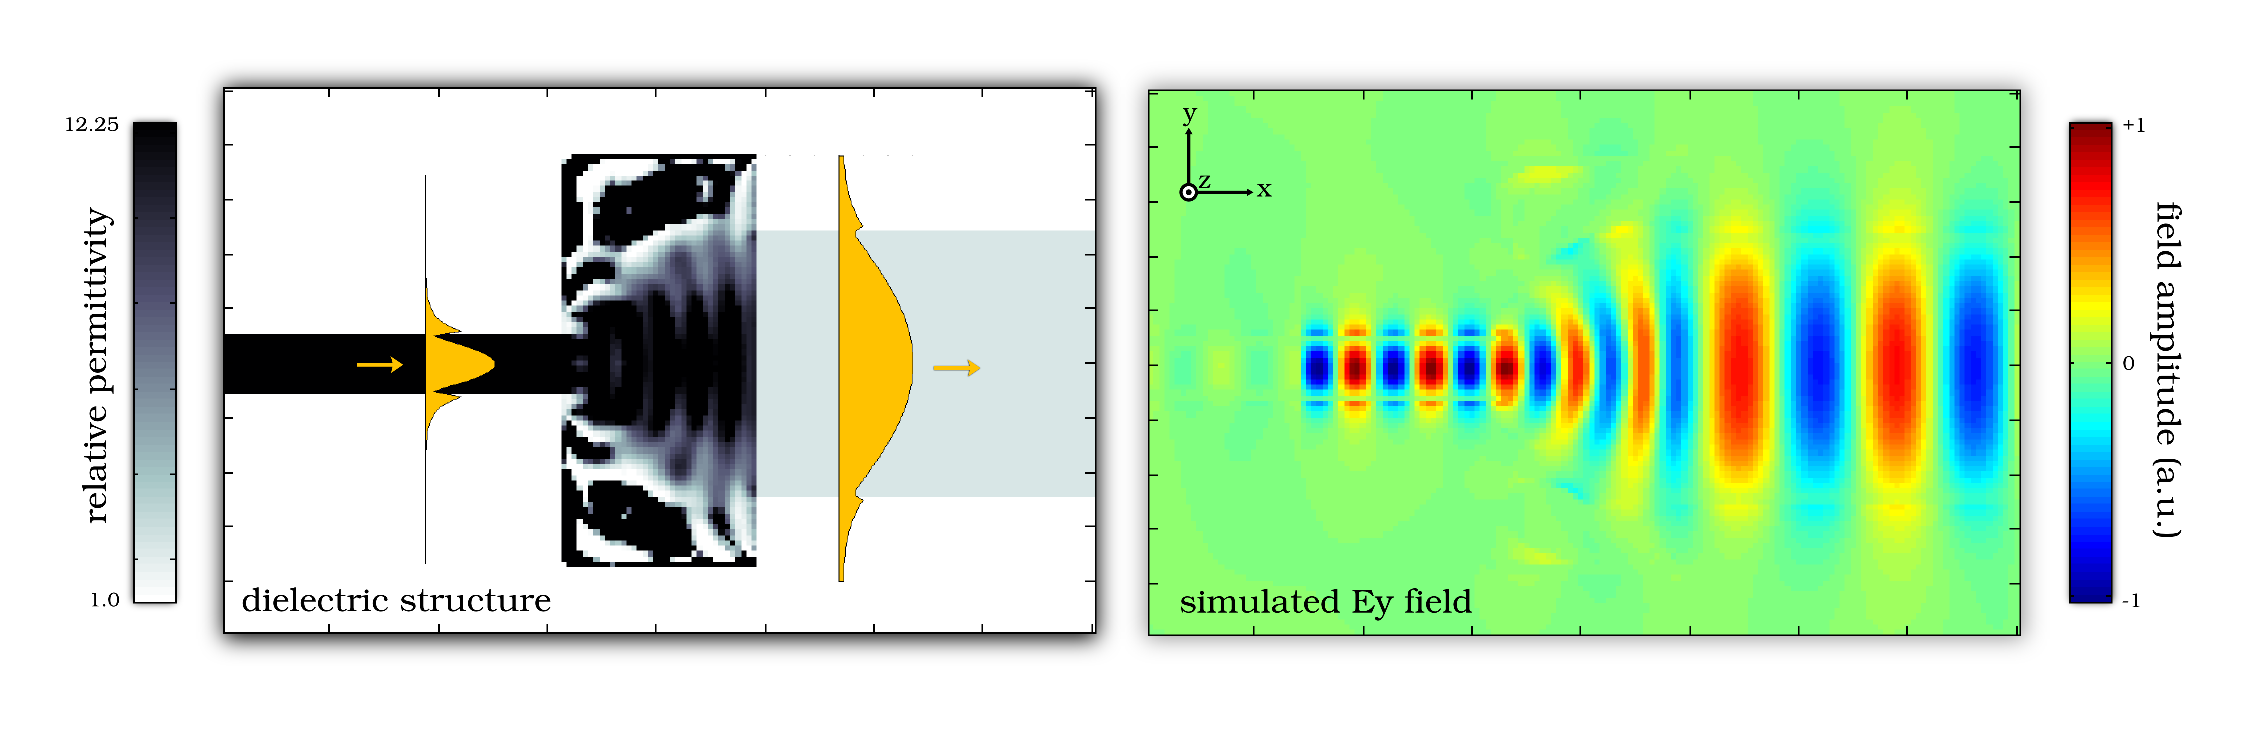
\includegraphics[width=\textwidth]{fiber} 
    \caption{Coupler from a narrow, high-index ($\epsilon=12.25$) waveguide to
        a wide, low-index ($\epsilon=2.25$) waveguide. 
        On the left, the dielectric structure of the coupler 
        and surrounding input and output waveguides are shown.
        The $H_z^\text{perfect}$ boundary values used as 
        the design objective are plotted on the left as well
        (top and bottom boundary values were set to zero).
        On the right, we show the simulation results used
        to compute the performance of the device.
        The coupler converts $96.3\%$ of the input power to the
        designated output mode.
        The device is also extremely compact, 
        convering only $36 \times 66$ grid points,
        where the vacuum wavelength is 42 grid points.
        Computation time was 20 minutes on a personal computer.}
    \label{fig:fiber}
\end{figure}
\begin{figure}[htbp]
    \centering
    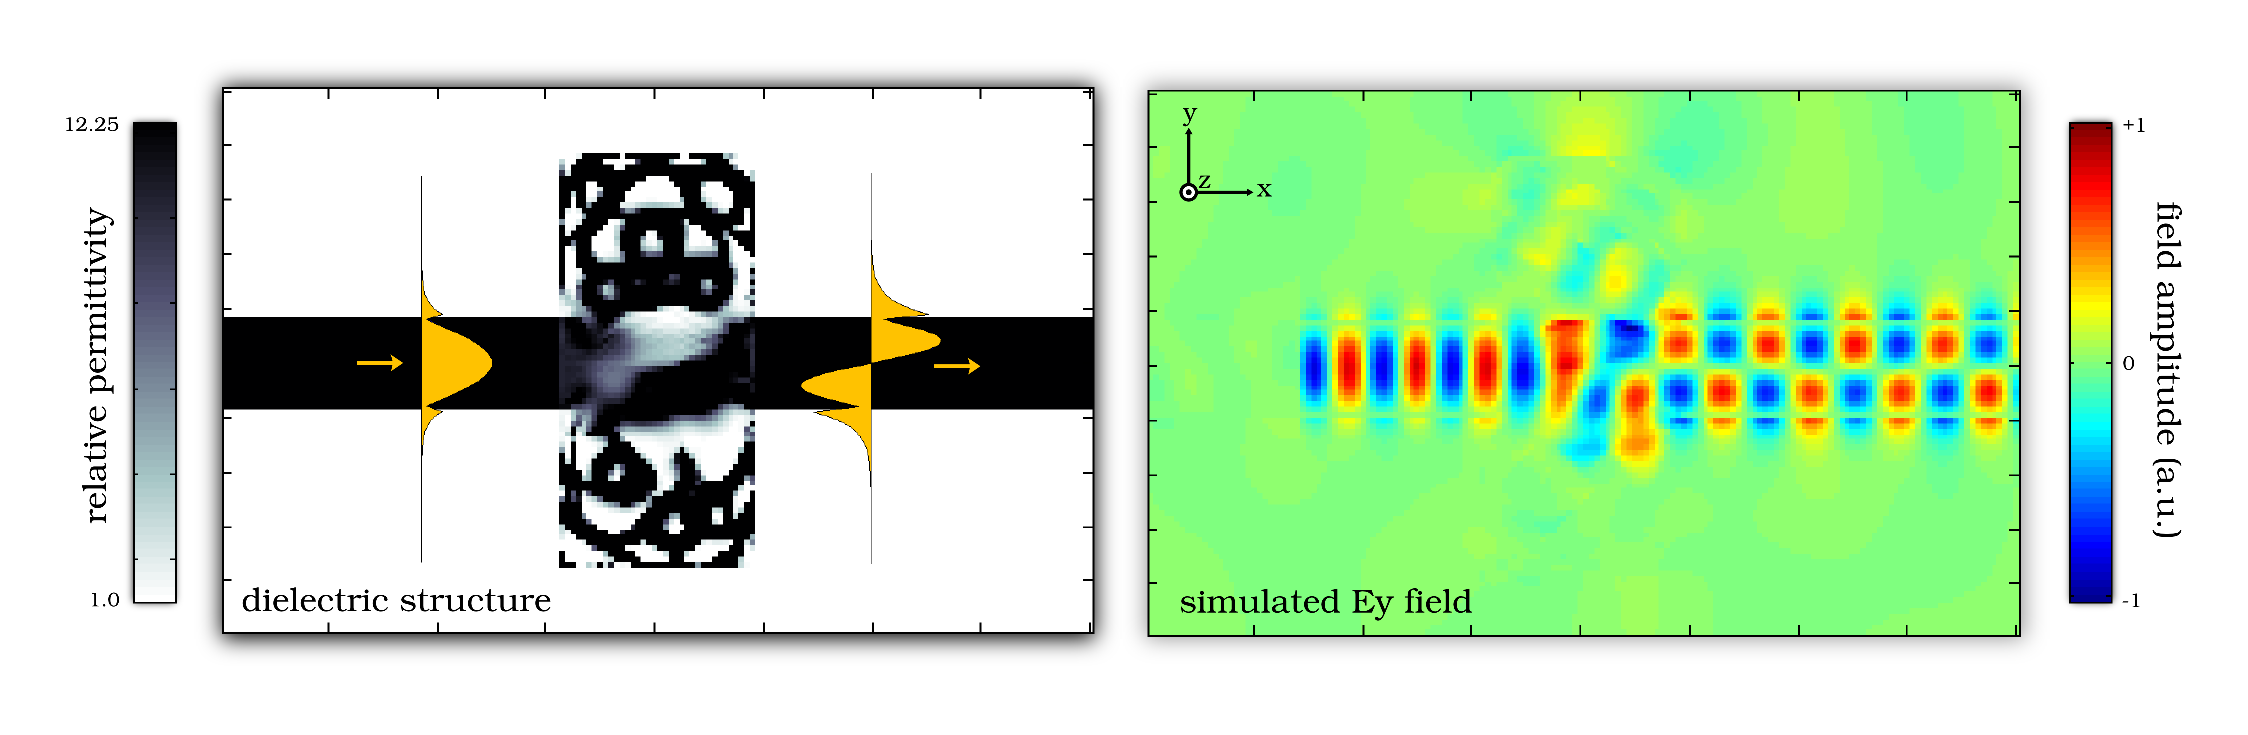
\includegraphics[width=\textwidth]{mode-conv} 
    \caption{Coupler that converts the fundamental waveguide mode to the
        second-order waveguide mode
        (a movie of the design progress is included as a
        supplementary material).
        This problem is quite difficult since the two modes are of 
        opposite symmetry.
        For example, adiabatic approaches cannot be applied to this case.
        However, our method produces a device 
        (which has the same dimensions and vacuum wavelength as Fig. 1) 
        with a coupling efficiency of $95.5\%$. 
        Computation time was 20 minutes on a personal computer.
        }
    \label{fig:mode}
    \end{figure}
\begin{figure}[htbp]
    \centering
    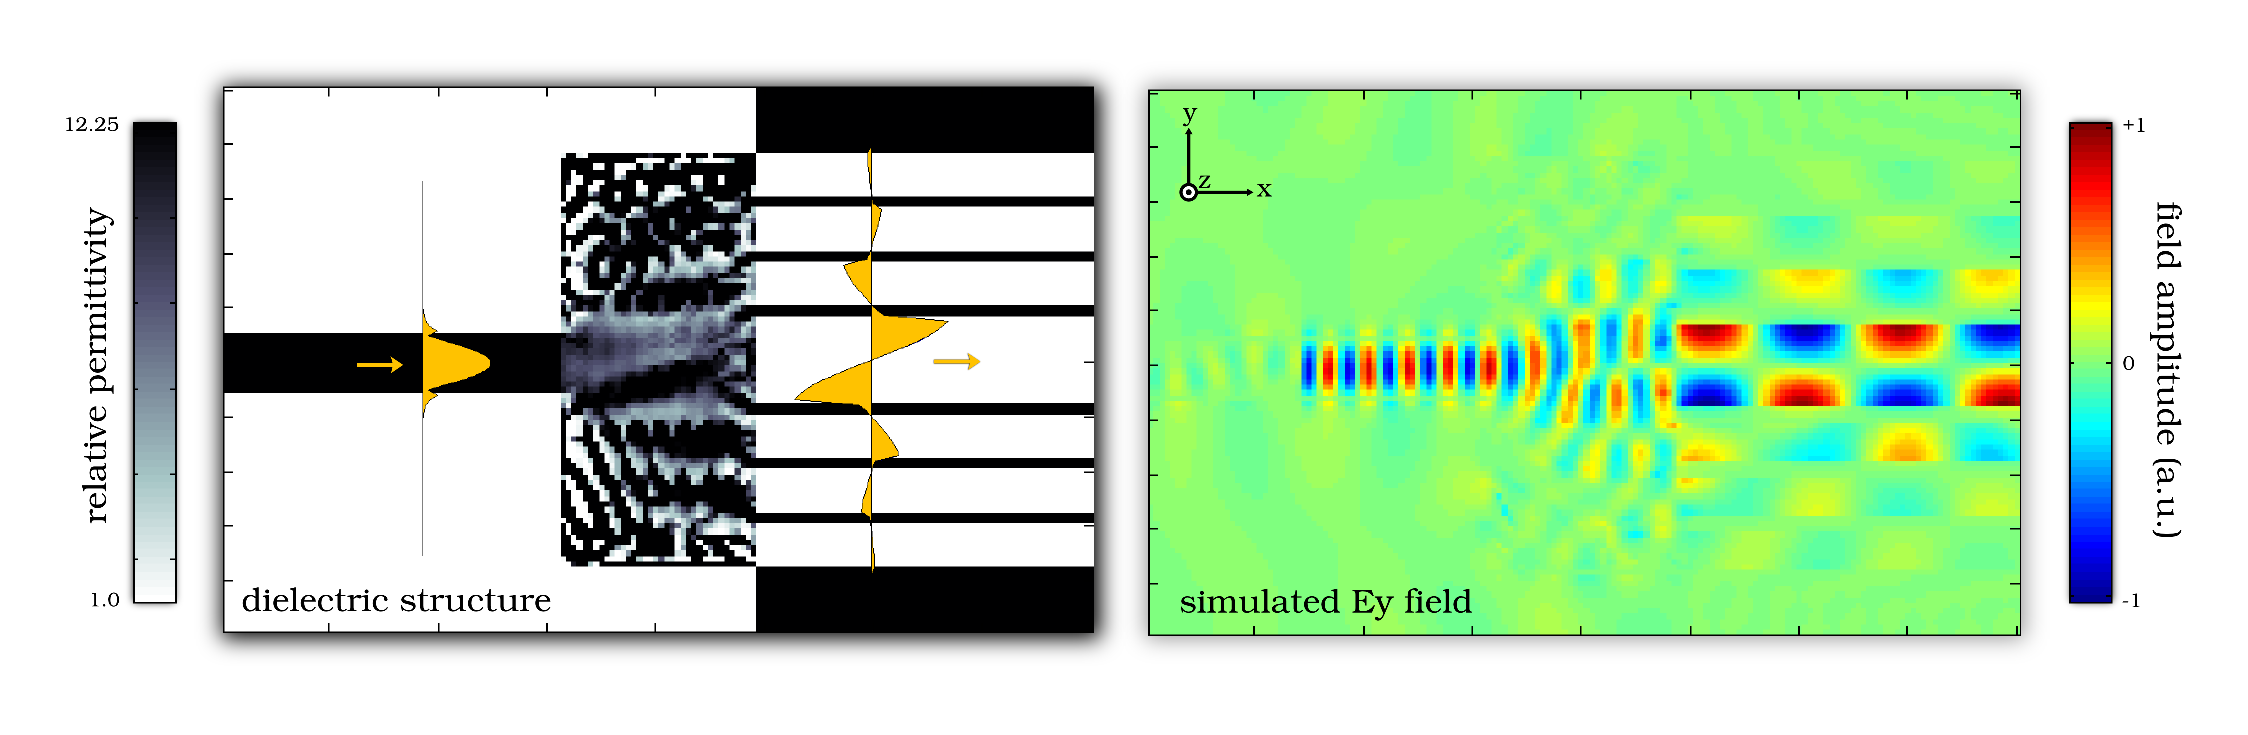
\includegraphics[width=\textwidth]{air-core}
    \caption{Coupler between a dielectric slab waveguide to 
        an air-core waveguide.
        Here, not only are the modes of opposite symmetry,
        but the output waveguide operates on a fundamentally different
        principle (distributed reflection) than the input waveguide 
        (index guided).
        The device still achieves an efficiency of $83.3\%$, demonstrating the
        versatility of our method.
        The vacuum wavelength is 25 grid points, 
        while the device footprint is still $36 \times 66$ grid points.
        Computation time was 20 minutes on a personal computer.
        }
        \label{fig:aircore}
\end{figure}

\section{Conclusion}
We develop a fundamentally new approach to designing physical structures,
    which we term ``objective-first'', 
    in that we choose to satisfy the design objective 
    even above satisfying the physical equation which governs its operation.
We show that such an approach drastically reduces the
    amount of computation required per iteration, and 
    performs well even with a non-functional initial design.

We then apply an objective-first approach to the design of 
    three practical nanophotonic waveguide couplers which are difficult, 
    at best, to solve with existing methods. 
We show that our method produces
    high-efficiency designs ($\sim 95\%$ efficiency) 
    in small footprints ($\sim 1$ square vacuum wavelength),
    is computationally fast (20 minutes on a single-core personal computer), and
    does not require trial-and-error, or even 
    a good starting design.\\


This work has been supported in part by the 
    AFOSR MURI for Complex and Robust On-chip Nanophotonics 
    (Dr. Gernot Pomrenke), grant number FA9550-09-1-0704.
The Matlab code used is available online\cite{code}.

\end{document}

